%
% assembly.tex
%
% Copyright (C) 2020 by SpaceLab.
%
% PC-104 Adapter Documentation
%
% This work is licensed under the Creative Commons Attribution-ShareAlike 4.0
% International License. To view a copy of this license,
% visit http://creativecommons.org/licenses/by-sa/4.0/.
%

%
% \brief Assembly instructions chapter.
%
% \author Gabriel Mariano Marcelino <gabriel.mm8@gmail.com>
%
% \institution Universidade Federal de Santa Catarina (UFSC)
%
% \version 2.0.0
%
% \date 2020/10/19
%

\chapter{Assembly Instructions} \label{ch:assembly}

This chapter presents the assembly instructions of the two boards and the interconnection cables between the top and bottom boards.

This project does not have sensible components (electrostatic or temperature), and no major care should be taken during the solder process. A recommended temperature of the soldering iron can be 350 $^{\circ}$C or lower.

\section{PCB Fabrication}

There is no major concerns about the PCBs fabrication. The boards were not designed to be fabricated without a solder mask, but if possible a Class 3 fabrication is recommended. A list with the recommended configuration can be seen in \autoref{tab:pcb-fabrication}.

\begin{table}[!h]
    \centering
    \begin{tabular}{L{0.5\columnwidth}L{0.5\columnwidth}}
        \toprule[1.5pt]
        \textbf{Parameter}      & \textbf{Value} \\
        \midrule
        Size                    & 86.26 $\times$ 91.9 mm \\
        Layers                  & 4 \\
        Thickness               & 1.6 mm \\
        Minimum Hole Size       & 0.3 mm \\
        Silkscreen Color        & White \\
        Surface Finish          & HASL with lead \\
        Via Process             & Tenting vias \\
        Material                & FR-4: TG150 \\
        Minimum Track/Spacing   & 6/6 mil \\
        Solder Mask Color       & Green \\
        Gold Fingers            & No \\
        Finish Copper           & 1 oz Cu (Inner Copper: 1 oz) \\
        \bottomrule[1.5pt]
    \end{tabular}
    \caption{Recommended configuration for fabrication.}
    \label{tab:pcb-fabrication}
\end{table}

\section{Top Board}

The instructions to assembly the top board are presented below:

\begin{enumerate}
    \item Solder the PicoBlade connectors (J1, J2, J3, J4, J5, J6, J7 and J8), beginning with the external connectors and moving to the center of the board, as can be seen in \autoref{fig:picoblades-instructions}.

\begin{figure}[!htb]
    \begin{center}
        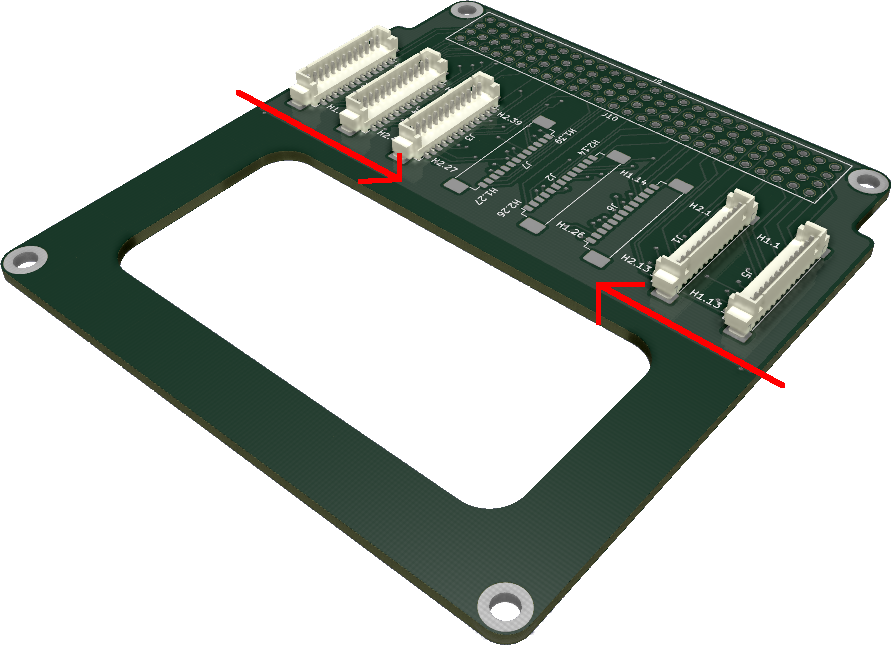
\includegraphics[width=0.6\columnwidth]{figures/picoblade-solder}
        \caption{Solder sequence of the PicoBlade connectors.}
        \label{fig:picoblades-instructions}
    \end{center}
\end{figure}

    \item Solder the PC-104 connectors (J9 and J10), taking care to keep the alignment of all the pins with the surface of the board, as can be seen in \autoref{fig:pc104-alignment}.

\begin{figure}[!htb]
    \begin{center}
        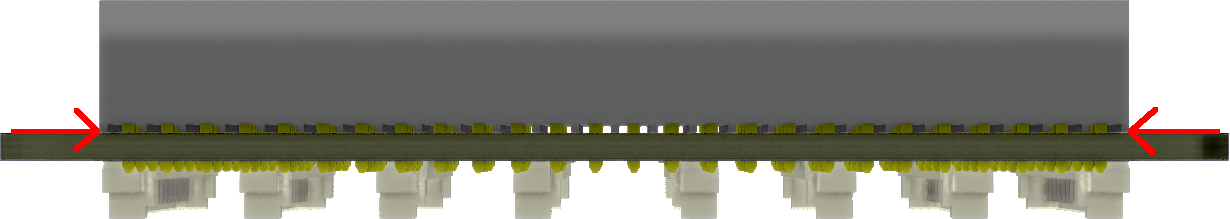
\includegraphics[width=0.7\columnwidth]{figures/pc104-alignment}
        \caption{Alignment of the PC-104 connectors.}
        \label{fig:pc104-alignment}
    \end{center}
\end{figure}
\end{enumerate}

\section{Bottom Board}

The same instructions apply to the bottom board:

\begin{enumerate}
    \item Solder the PicoBlade connectors (J1, J2, J3, J4, J5, J6, J7 and J8), beginning with the external connectors and moving to the center of the board, as can be seen in \autoref{fig:picoblades-instructions}.
    \item Solder the PC-104 connectors (J9 and J10), taking care to keep the alignment of all the pins with the surface of the board, as can be seen in \autoref{fig:pc104-alignment}.
\end{enumerate}

\section{Cables}

For now, there is no assembled cables with 13 wires available to buy. So, a custom set of cables is required to connect the top and bottom boards.

The instructions to assembly these custom cables are presented below:

\begin{enumerate}
    \item Remove all wiring housing from 15134-1401.
    \item Mount the wires in 51021-1300.
    \item As 15134-1401 is a cable assembly with 14 wires and 51021-1300 is a connector with 13 positions, one wire per cable will remain.
\end{enumerate}
